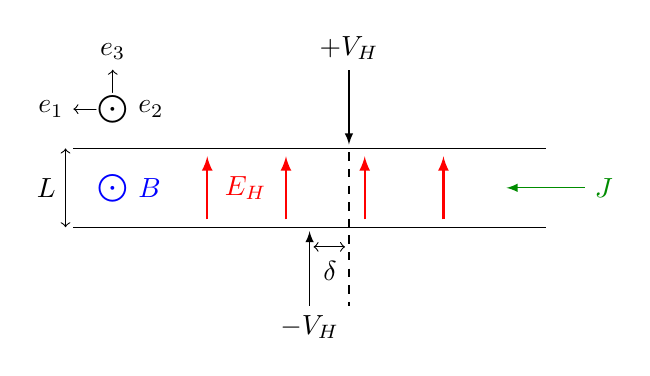
\begin{tikzpicture}
    \draw[<->] (0,1.5) node[left] {$\vu{e}_1$} -| (0.5,2) node[above] {$\vu{e}_3$};
    \draw (0.7,1.5) node[right] {$\vu{e}_2$};
    \filldraw[white] (0.5, 1.5) circle (0.2) node[black] {$\mathbf{\bigodot}$};
    \draw (0,0) -- (6,0) (0,1) -- (6,1);
    \draw[latex-, black!45!green] (5.5, 0.5) to (6.5,0.5) node[right] {$\va{J}$};
    \foreach \i in {1,...,4} \draw[-latex,thick, red] (\i+0.7,0.1) to (\i+0.7,0.9)
    ;
    \draw[red] (1.8,0.5) node[right] {$\va{E}_H$};
    \filldraw[white] (0.5, 0.5) circle (0.2) node[blue] {$\mathbf{\bigodot}$};
    \draw[blue] (0.7,0.5) node[right] {$\va{B}$};
    \draw[latex-] (3,-0.05) to (3, -1) node[below]{$-V_H$};
    \draw[latex-] (3.5,1.05) to (3.5, 2) node[above]{$+V_H$};
    \draw[dashed] (3.5,0.95) to (3.5,-1);
    \draw (3.05, -0.55) node[right] {$\delta$};
    \draw[<->] (3.05, -1+0.75) to (3.45,-1+0.75);
    \draw[<->] (-0.1,0) to (-0.1,1);
    \draw (-0.1,0.5) node[left] {$L$}
    ;
\end{tikzpicture}